\documentclass[border=12pt]{standalone}
\usepackage[european]{circuitikz}
\begin{document}
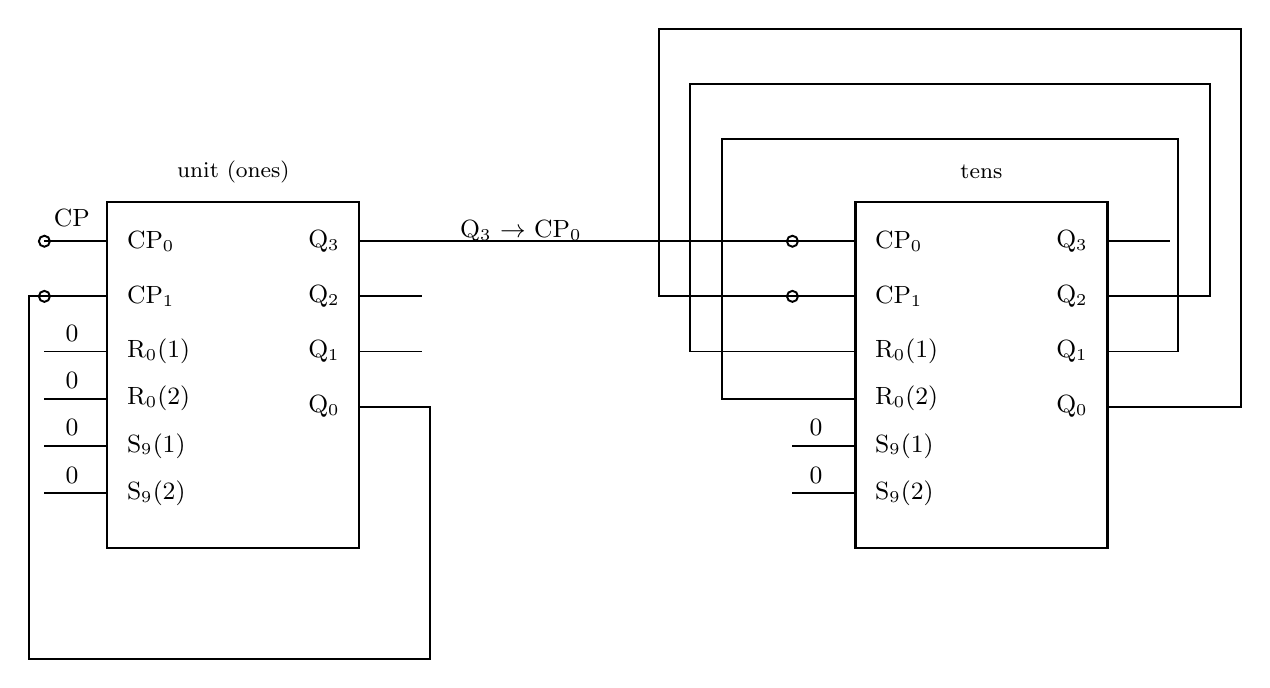
\begin{tikzpicture}[line width=0.7pt, font=\small]

% 片体 3.2 x 4.4。左引脚端 bx-0.8，右引脚端 bx+4.0
%
% 片内反馈统一从框上方绕行（三条嵌套通道，导线交叉落在片体上方的空白区，
% 不穿框体、不压任何文字）：
%   右竖通道 bx+4.1 / +4.4 / +4.7；顶部横线 y=5.2 / 5.8 / 6.4；左竖通道 bx-1.0 / -1.3 / -1.6
% 跨片 Q3→CP0 走两片之间的 y=3.9 水平直线（片 1 右端 4.0 → 片 2 左端 8.7）
\newcommand{\chipbase}[2]{%
  \draw[thick] (#1,0) rectangle (#1+3.2,4.4);
  \node[font=\footnotesize] at (#1+1.6,4.78) {#2};
  \foreach \y/\n in {3.9/{CP$_0$},3.2/{CP$_1$},2.5/{R$_0$(1)},1.9/{R$_0$(2)},1.3/{S$_9$(1)},0.7/{S$_9$(2)}} {%
    \node[font=\small, anchor=west] at (#1+0.12,\y) {\n};
    \draw (#1,\y) -- (#1-0.8,\y);
  }
  \draw (#1-0.8,3.9) circle (0.07);
  \draw (#1-0.8,3.2) circle (0.07);
  \foreach \y/\n in {3.9/{Q$_3$},3.2/{Q$_2$},2.5/{Q$_1$},1.8/{Q$_0$}} {%
    \node[font=\small, anchor=east] at (#1+3.08,\y) {\n};
    \draw (#1+3.2,\y) -- (#1+4.0,\y);
  }
}

% ── 片 1（个位）：CP0 接外部输入；CP1←本片 Q0；R0、S9 全部接地 ──
\chipbase{0}{unit (ones)}
\node[font=\small, anchor=south] at (-0.45,3.96) {CP};
\foreach \y in {2.5,1.9,1.3,0.7} {\node[font=\small, anchor=south] at (-0.45,\y) {0};}
\draw (4.0,1.8) -- (4.1,1.8) -- (4.1,-1.4) -- (-1.0,-1.4) -- (-1.0,3.2) -- (-0.8,3.2);

% ── 片 2（十位）：CP1←Q0；R0(1)←Q2；R0(2)←Q1；S9 接地 ──
\chipbase{9.5}{tens}
\foreach \y in {1.3,0.7} {\node[font=\small, anchor=south] at (9.0,\y) {0};}
\draw (13.5,1.8) -- (14.4,1.8) -- (14.4,6.6) -- (7.0,6.6) -- (7.0,3.2) -- (8.7,3.2);
\draw (13.5,3.2) -- (14.0,3.2) -- (14.0,5.9) -- (7.4,5.9) -- (7.4,2.5) -- (8.7,2.5);
\draw (13.5,2.5) -- (13.6,2.5) -- (13.6,5.2) -- (7.8,5.2) -- (7.8,1.9) -- (8.7,1.9);

% ── 跨片：片 1 的 Q3 → 片 2 的 CP0 ──
\draw (4.0,3.9) -- (8.7,3.9);
\node[font=\small, anchor=west] at (4.35,4.02) {Q$_3$ $\to$ CP$_0$};

\end{tikzpicture}
\end{document}
